\section{Implementation}\label{sec:impl}
In this section, we elaborate on how we collect data for training, the specific parameters we choose for the two orthogonal neural networks, and the software/hardware environment we use.

\paragraph{Data generation}
For each scene, we generate two datasets separately for training foveal and periphery networks. The foveal dataset is composed of $256\times256$ images rendered at different views with 20 deg field-of-view, while the periphery dataset uses 45 deg field-of-view to rendering. The view translations ($\rayo$) are sampled every $5$ cm on each axis. The rotations ($\camDir$) are sampled so that adjacent samples are seamlessly connected with no overlap.
% \nothing{
% %\paragraph{Input encoding}
% Similar to \cite{mildenhall2020nerf}, we also extend the input dimensions ($d=3$) to a higher dimensional ($d=60$) for training. 
% \nothing{This is achieved via coding the input as:
% \begin{align}
% \iota (p) = (\sin(2^0 p), \cos(2^0 p), ..., \sin(2^{L-1}p, \cos(2^{L-1}p))
% \label{eqn:inputencode}
% \end{align}
% The function $\iota (\cdot)$ is applied to dimension of $\SpatialPt=(r_\SpatialPt,\theta_\SpatialPt, \phi_\SpatialPt)$.
% In our experiment we choose $L=10$.\qisun{What is $L$?}\dnc{It's an encoding parameter for input. maps 3D input to $R^{6L}$ space, as \autoref{eqn:inputencode} shows}
% }}
\paragraph{Optimized network parameters}
Guided by the latency-quality joint optimization described in \Cref{sec:method:optimization}, we implemented the foveal network with $\mlpLayerNum=4$, $\mlpChannelNum=128$ and $\sphereNum = 32$. For the periphery neural network, the values are $\mlpLayerNum=4$, $\mlpChannelNum=96$ and $\sphereNum = 16$. These optimized parameters achieve a proper balance between quality and latency, as shown in \Cref{fig:results:comparison} and \Cref{tbl:ablation}.

\paragraph{Ray marching bounding}
We bound the ray marching within region that $\mathbf{\sphereRadius}$ are sampled in, thus has impact on $\sparseError$ in \Cref{eq:sparseError}. As shown in \Cref{fig:impl:bounding:off}, results with infinite upper bounding ($\sphereRadius\in[\sphereRadius_{near},+\infty)$ incur blurry and ghosting artifacts due to larger $\sparseError$. In contrast, limited bounding significantly improves the quality (\Cref{fig:impl:bounding:on}). %The bounding range, together with $\sphereNum$, $\mlpLayerNum$ and $\mlpChannelNum$, are determined by a spatial-temporal optimization, as detailed in \Cref{sec:method:optimization}.
\begin{figure}
    \centering
    \subfloat[w/o bounding]{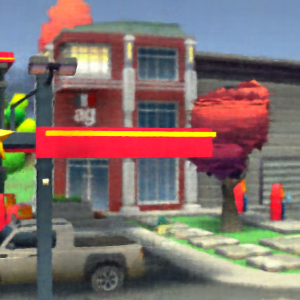
\includegraphics[width = 0.47\linewidth]{TOG/figs/depth_without_bound.png}}\hspace{1em}
    \subfloat[w bounding]{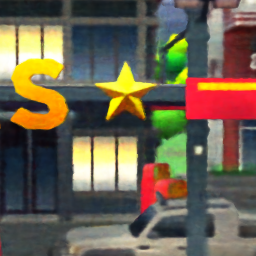
\includegraphics[width = 0.47\linewidth]{TOG/figs/depth_with_bound.png}}
    \Caption{Comparison of ray marching bounding.}
    {%
    }
    \label{fig:method:bounding}
\end{figure}
\begin{figure*}[htb]
    \centering
    \begin{minipage}{0.32\linewidth} %full res
        \subfloat[gas scene(\textbf{GT})]{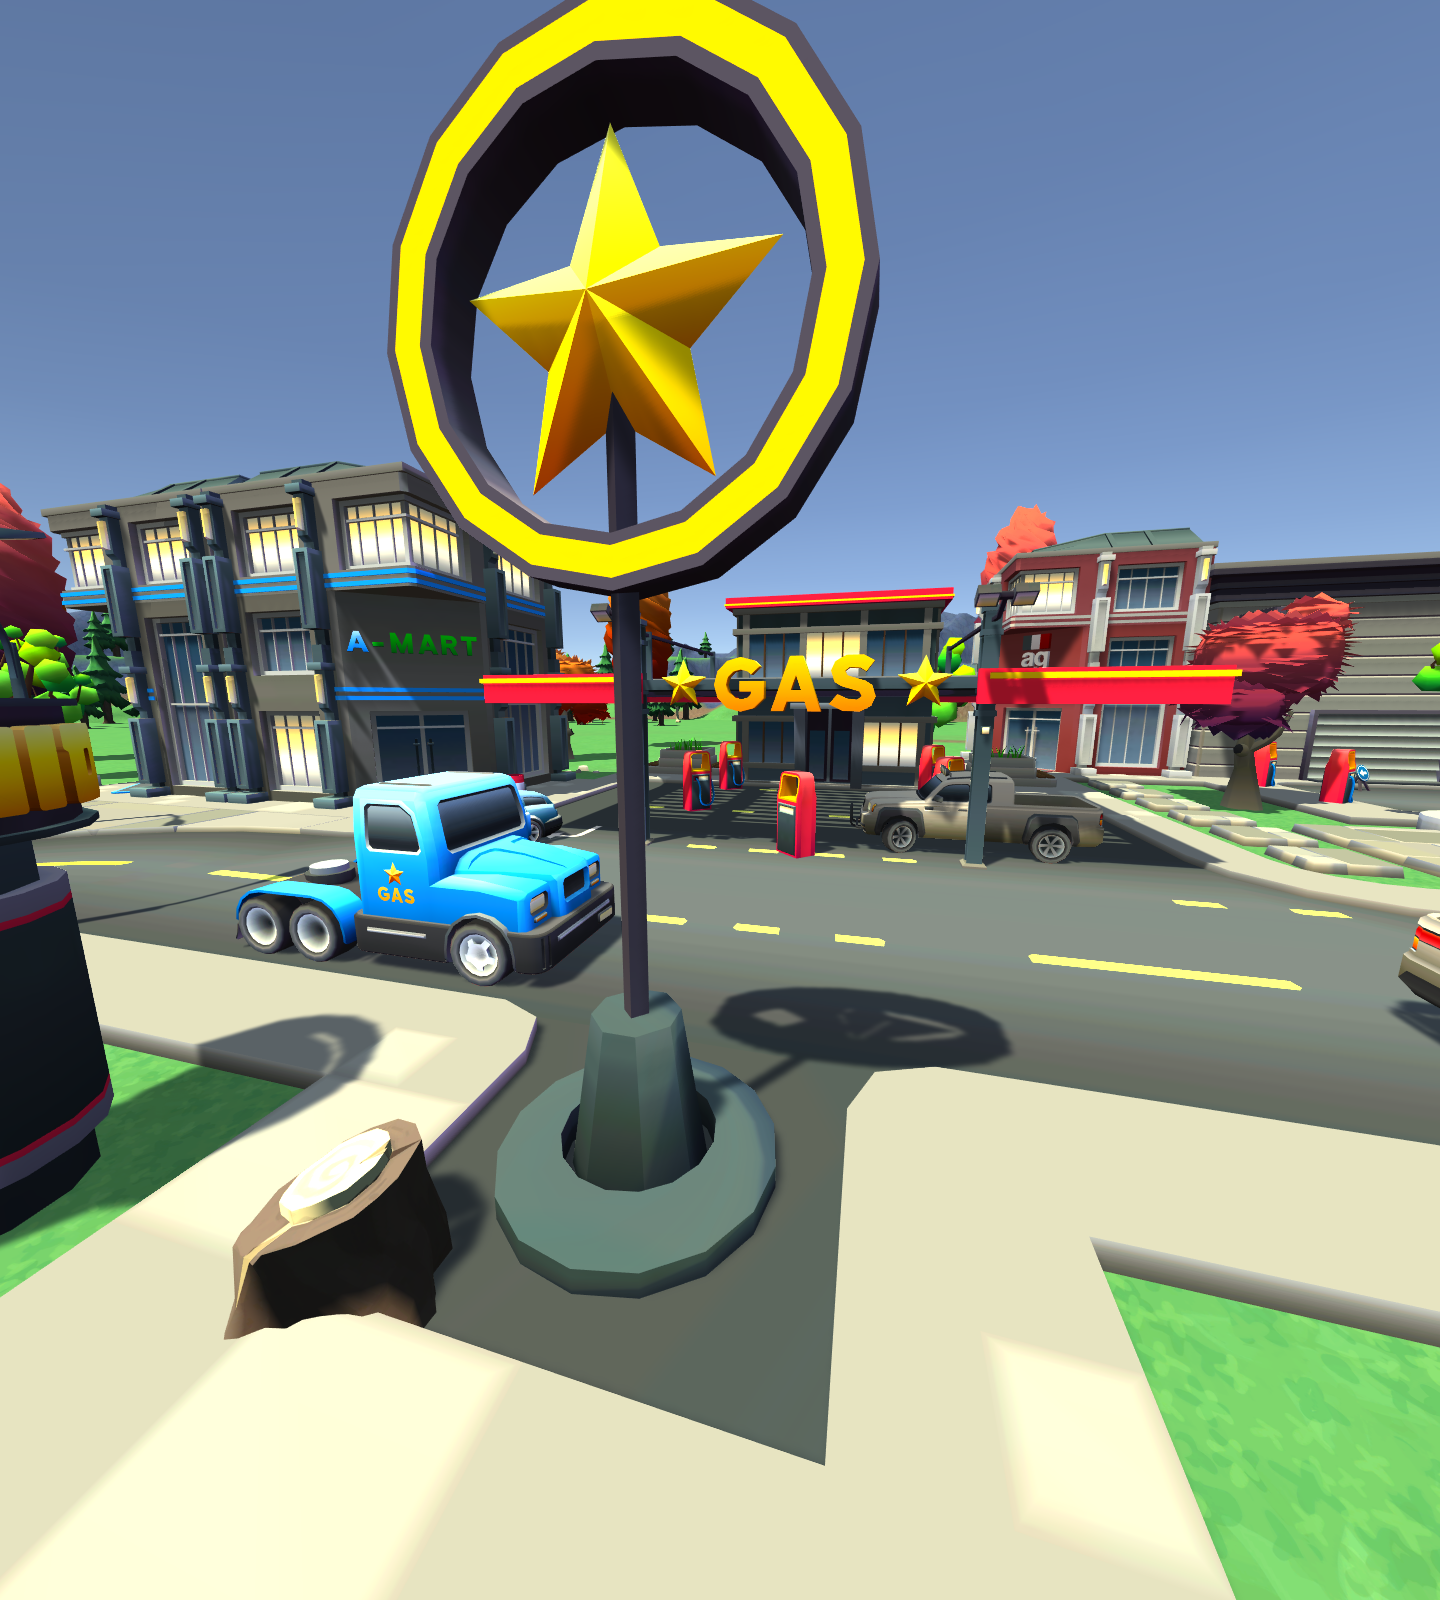
\includegraphics[width=0.96\linewidth]{TOG/figs/gas_gt4.png}}
        
        \subfloat[minecraft scene(\textbf{GT})]{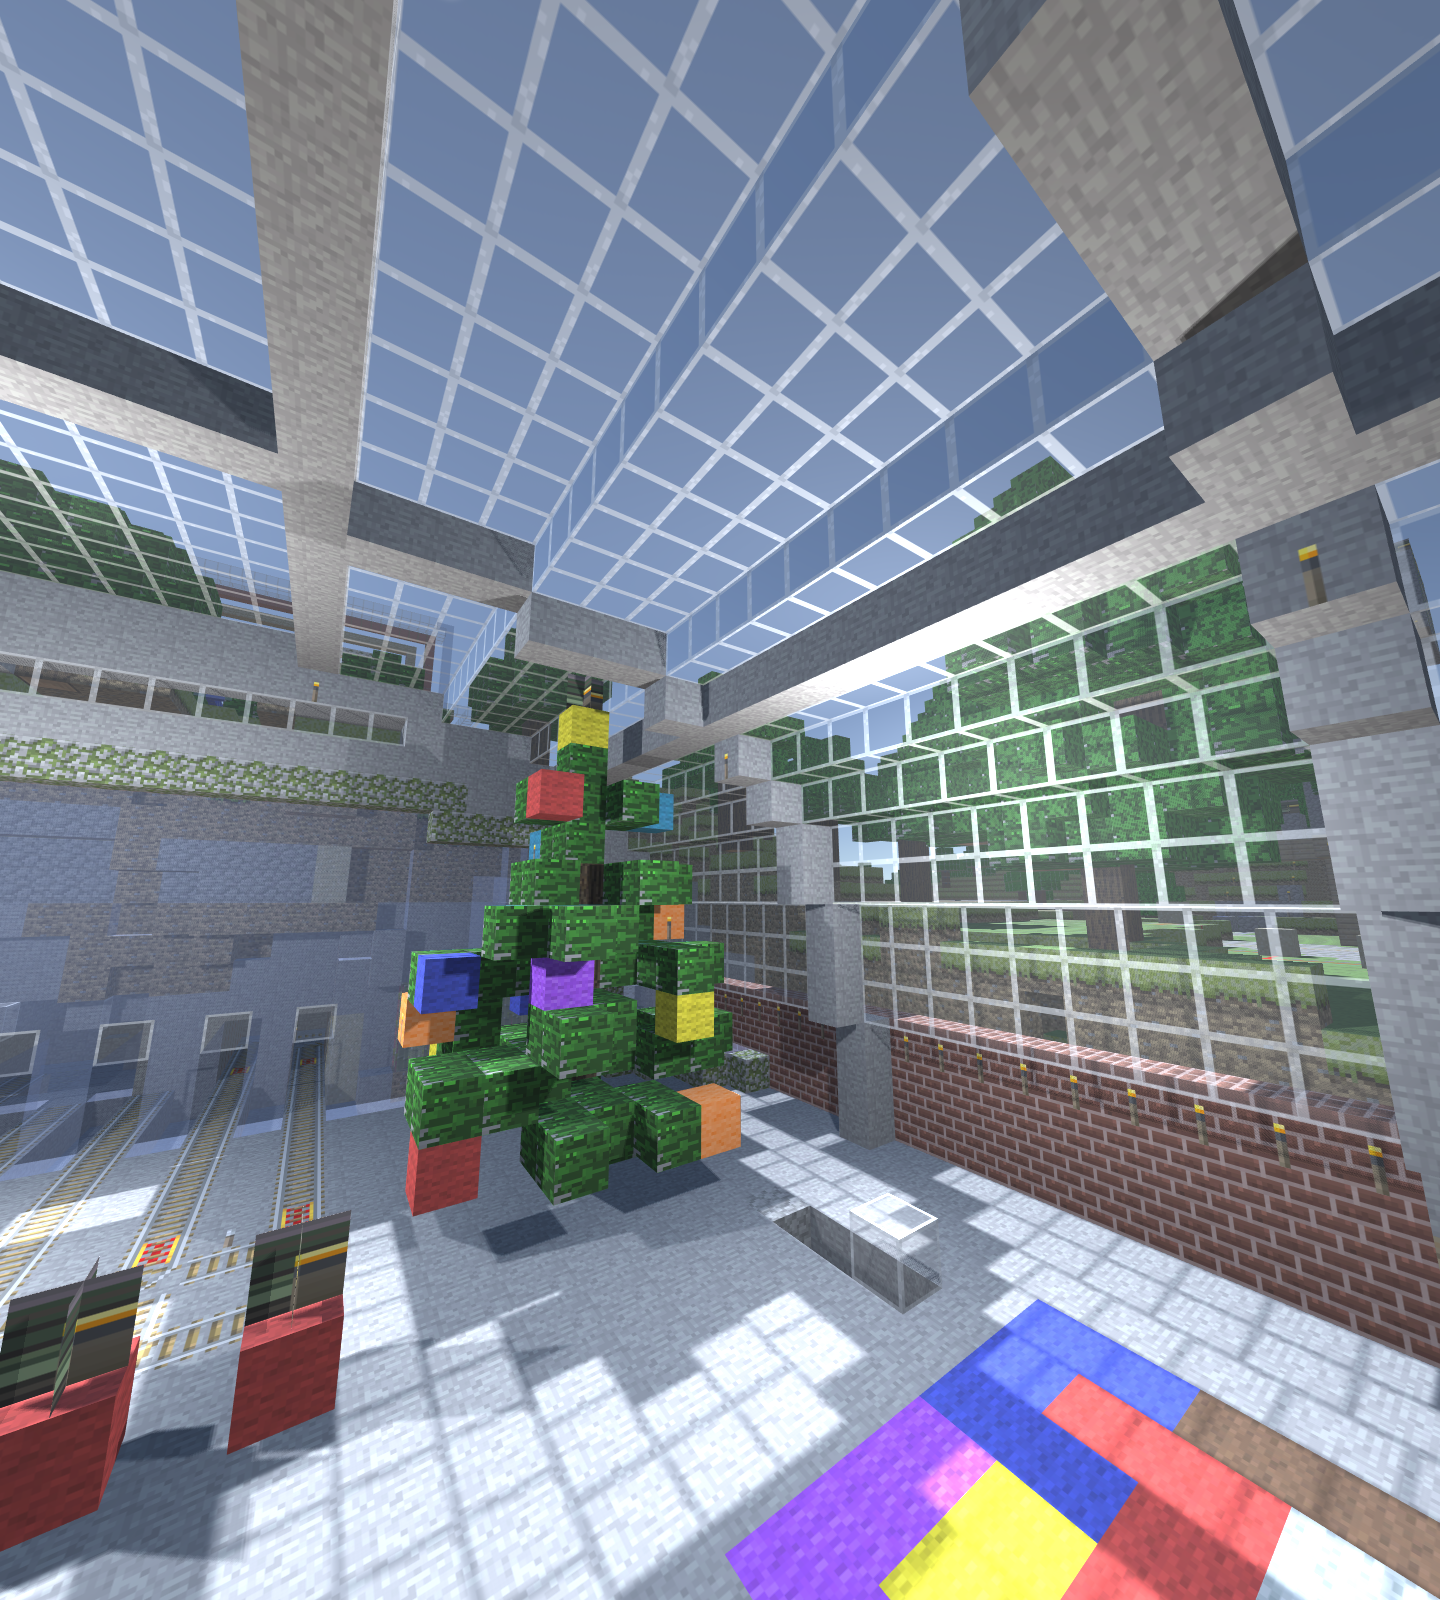
\includegraphics[width=0.96\linewidth]{TOG/figs/mc_gt3.png}}
        
        \subfloat[bedroom scene(\textbf{GT})]{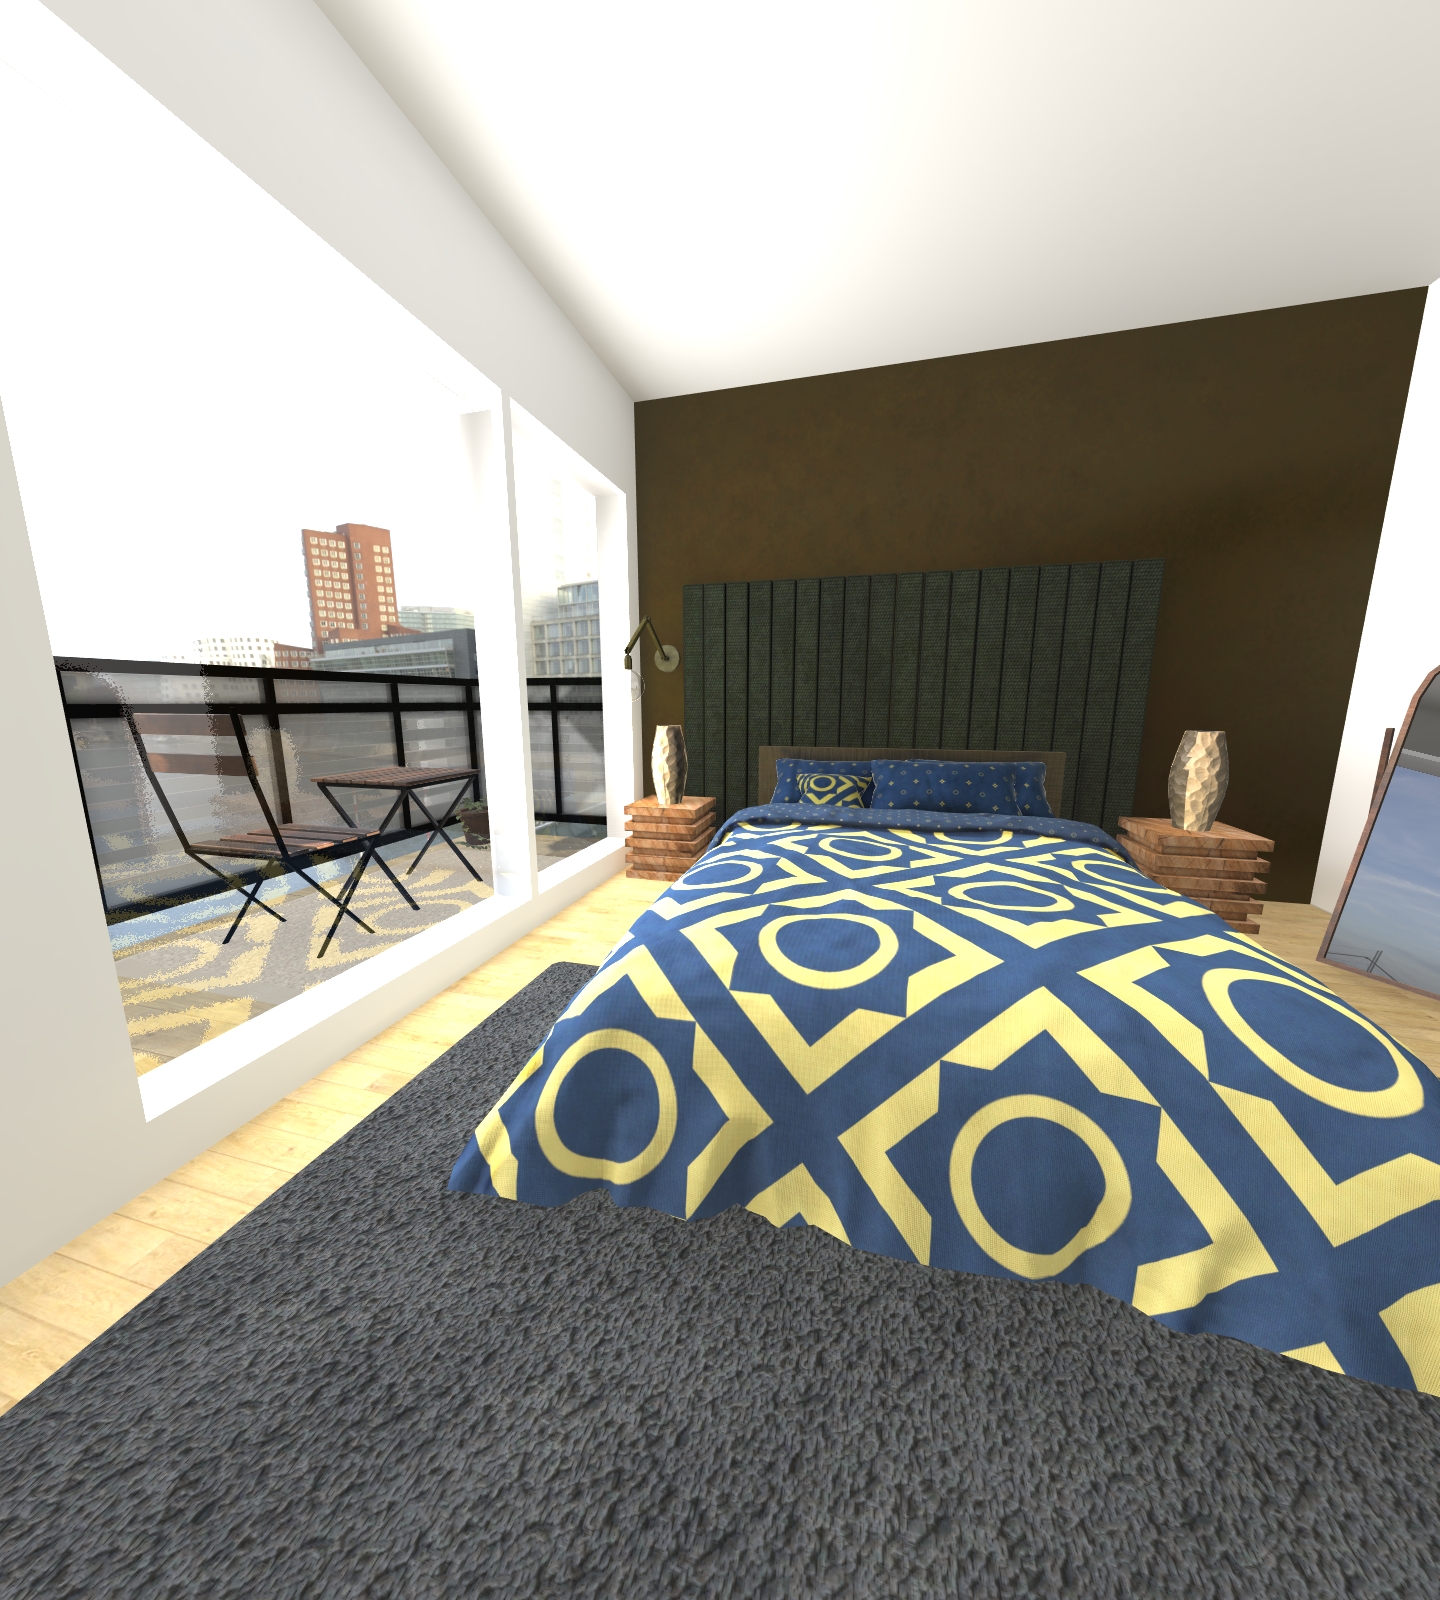
\includegraphics[width=0.96\linewidth]{TOG/figs/bed_gt0.png}}
    \end{minipage}
    \begin{minipage}{0.32\linewidth} %ours
        \subfloat[gas scene (\textbf{OUR})]{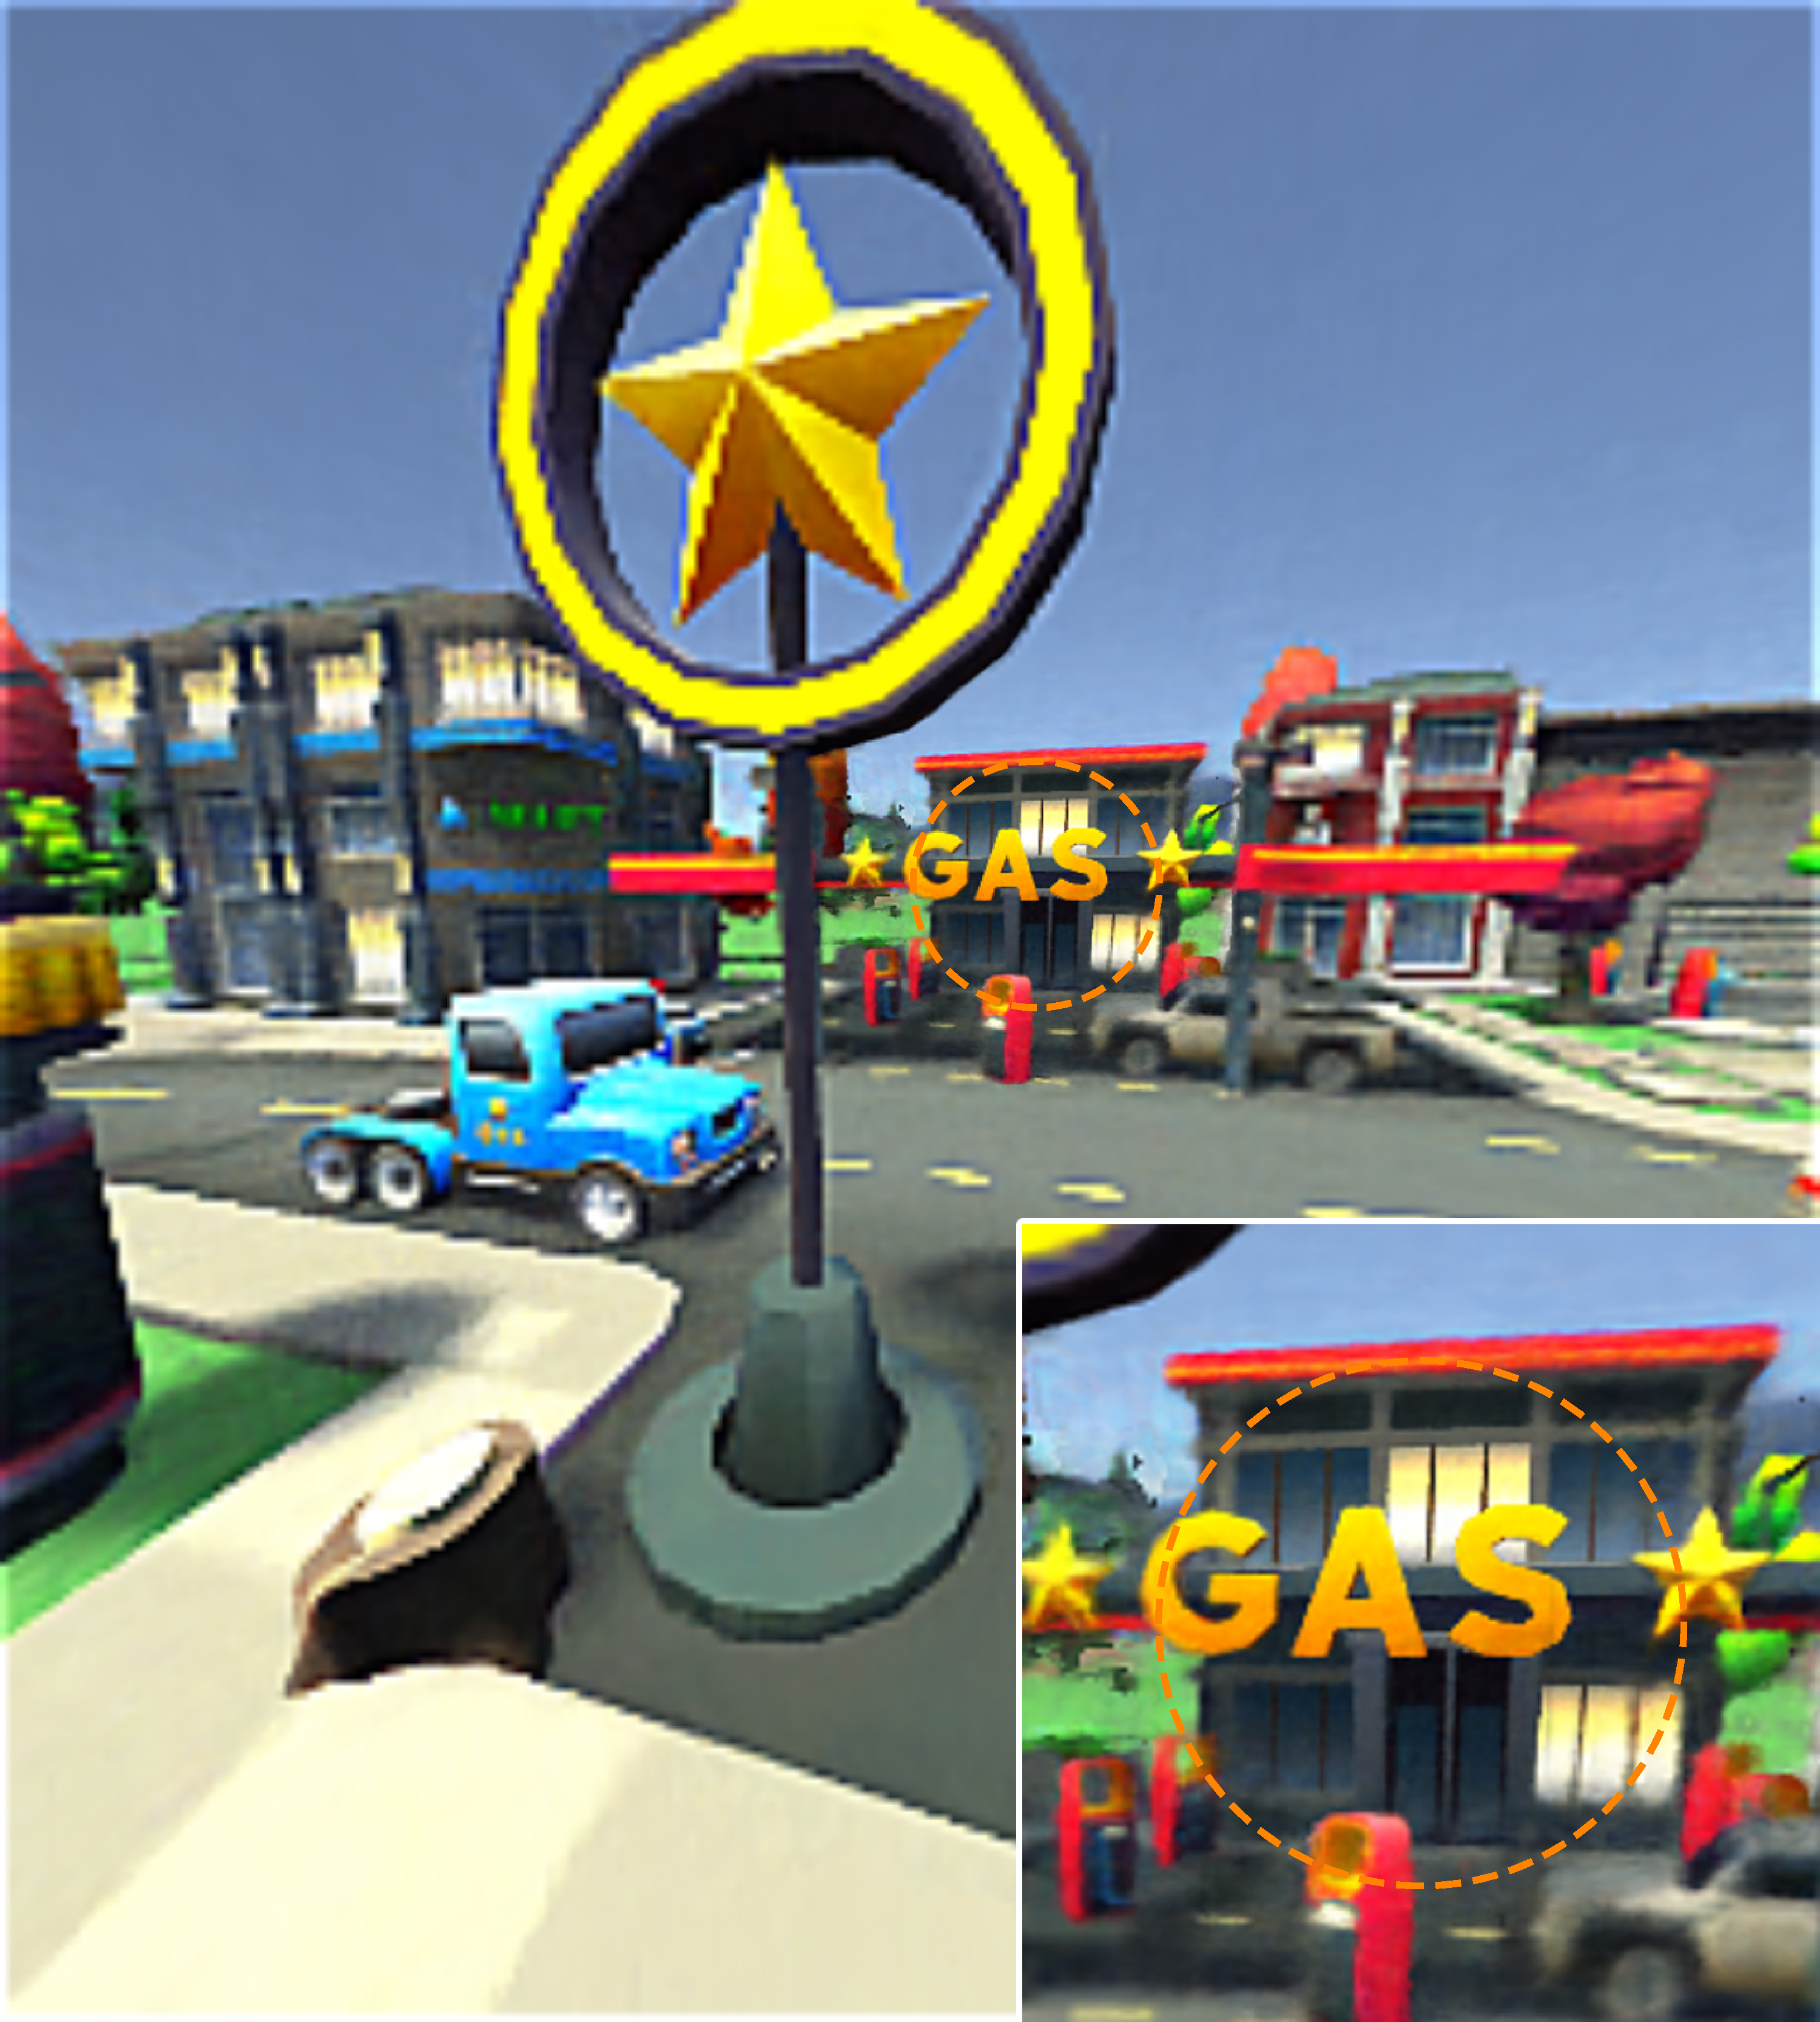
\includegraphics[width=0.96\linewidth]{TOG/figs/gas_our4_inset.pdf}}
        
        \subfloat[minecraft scene (\textbf{OUR})]{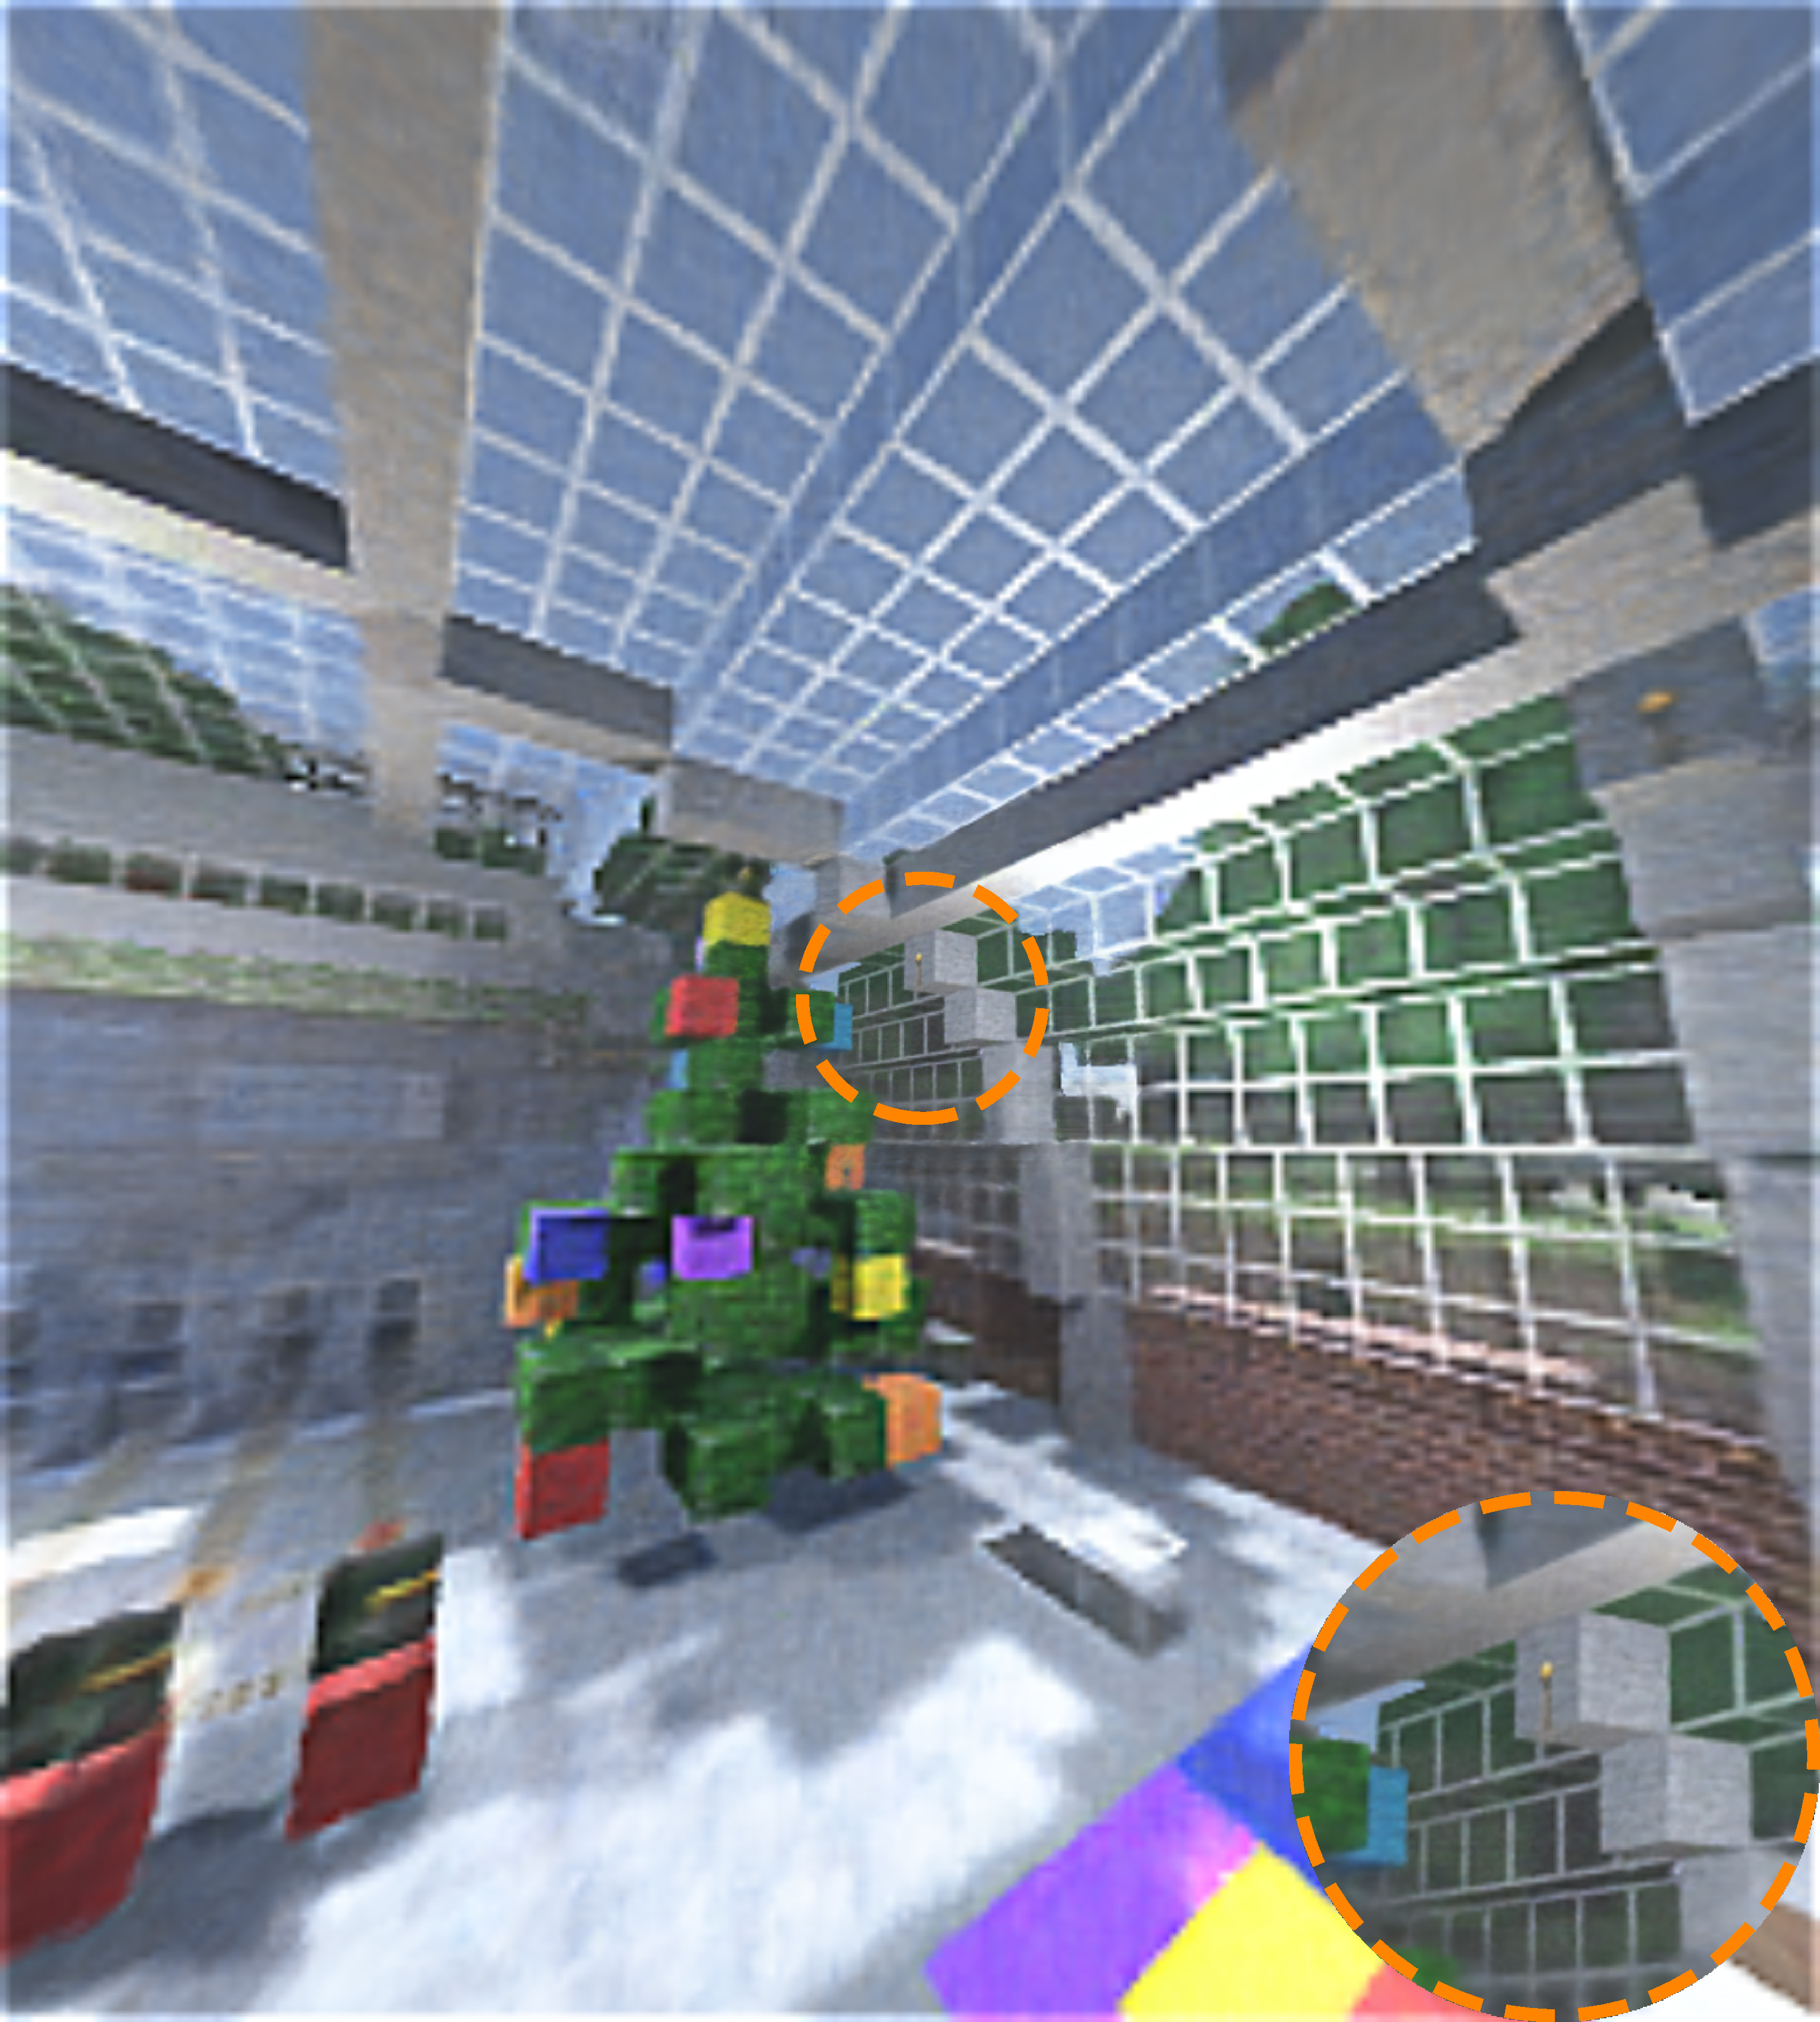
\includegraphics[width=0.96\linewidth]{TOG/figs/mc_our3_inset.pdf}}
        
        \subfloat[bedroom scene (\textbf{OUR})]{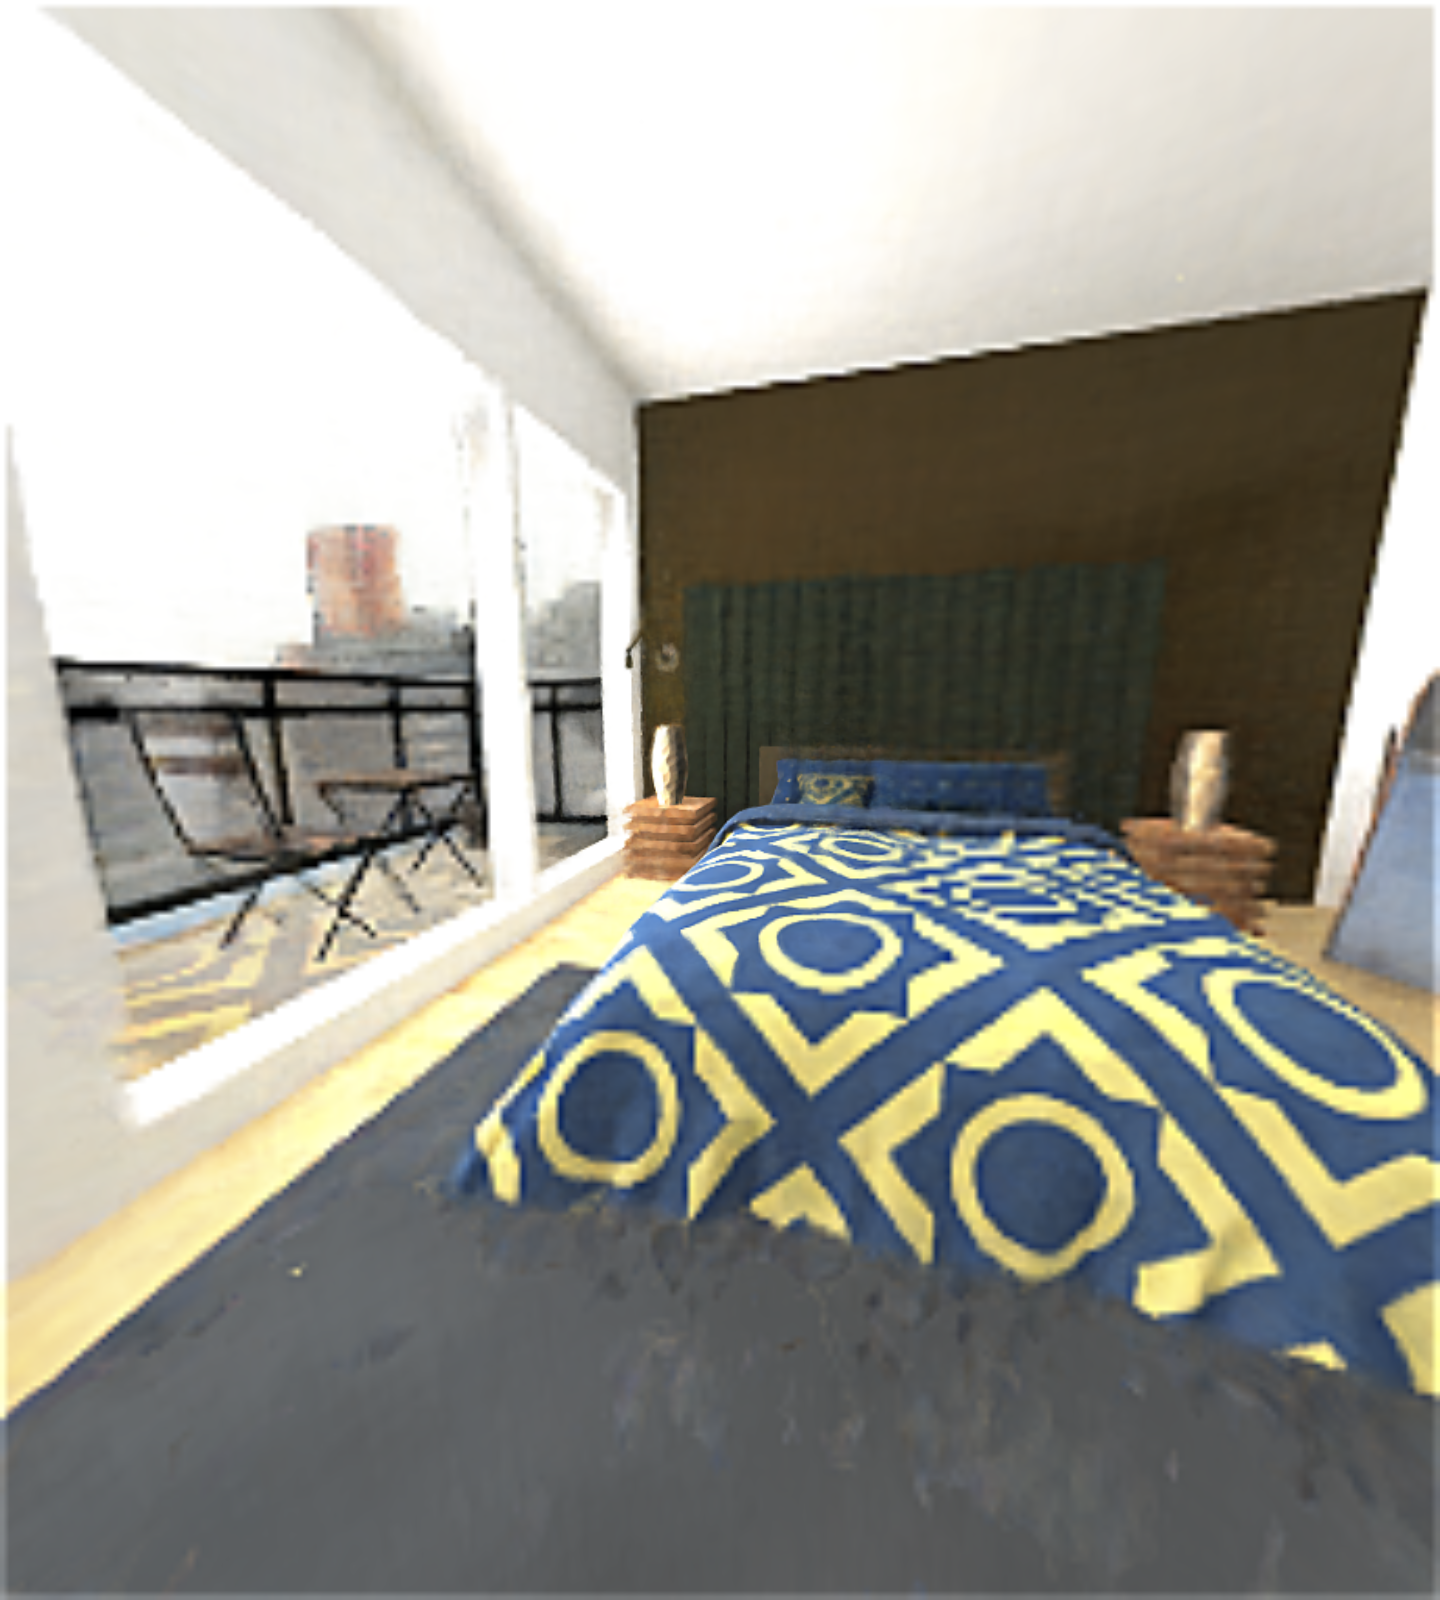
\includegraphics[width=0.96\linewidth]{TOG/figs/bed_our0.png}}               
    \end{minipage}
    \begin{minipage}{0.32\linewidth} % NERF
        \subfloat[gas scene (\textbf{NeRF})]{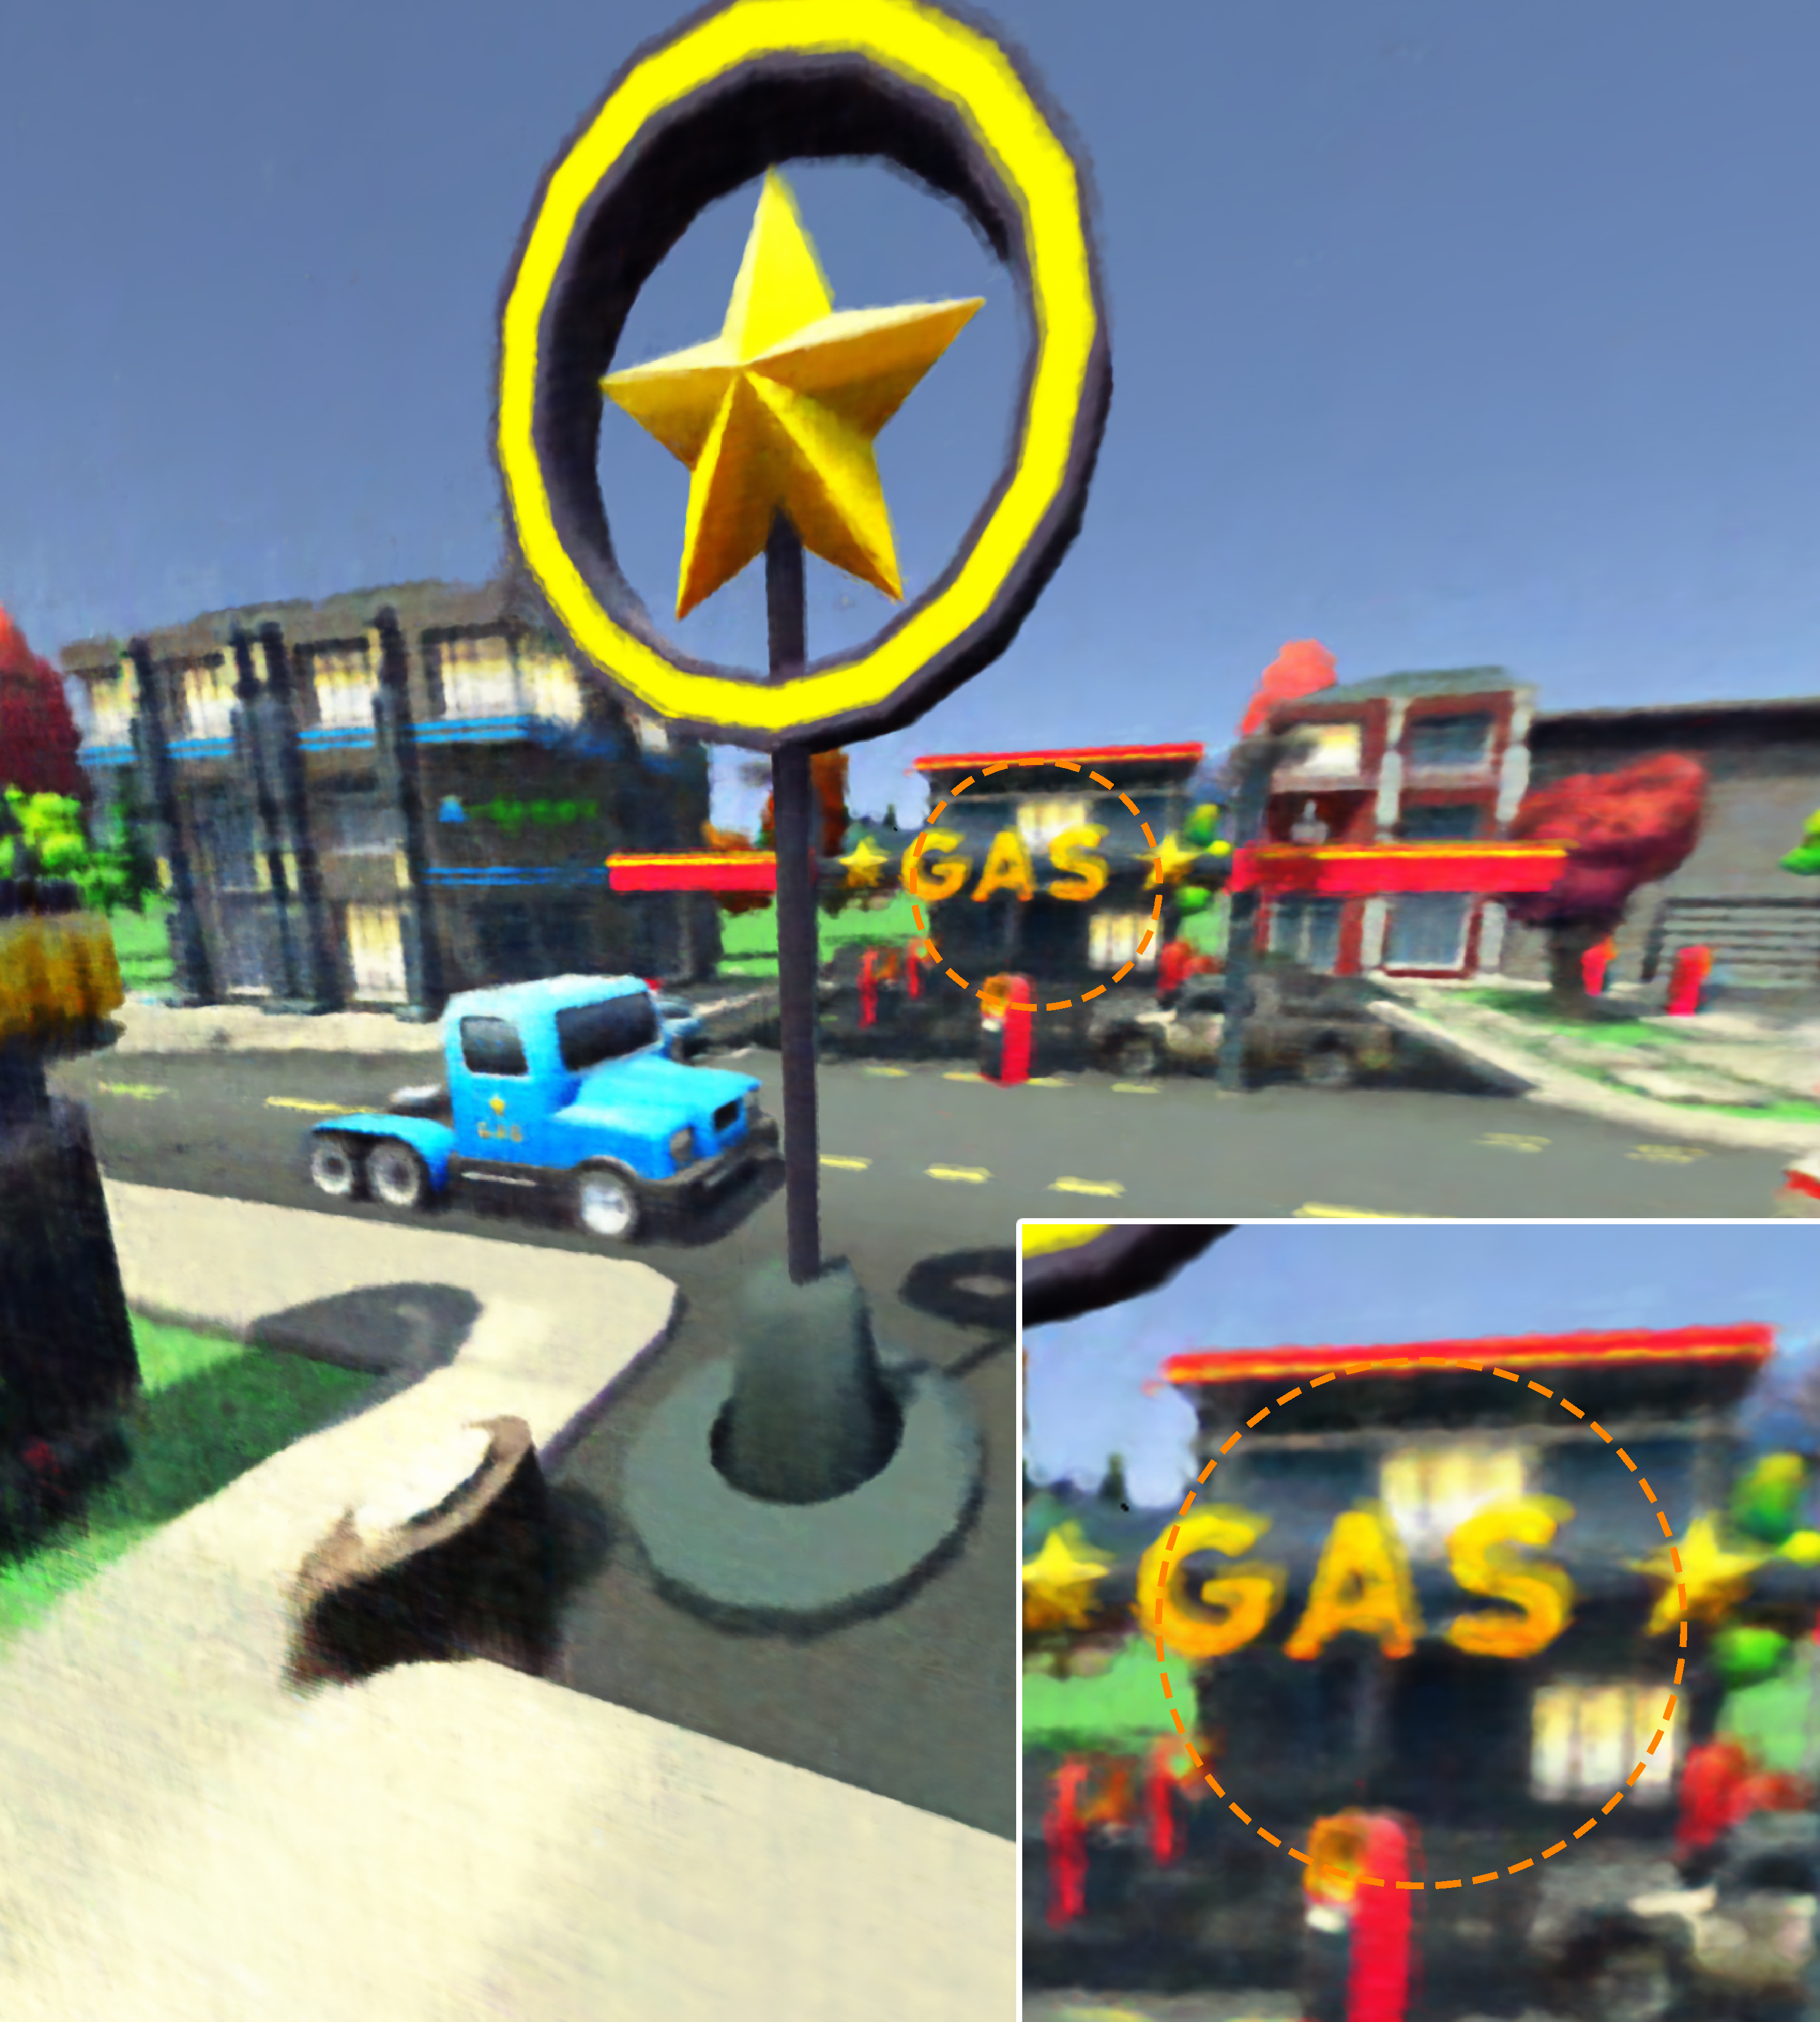
\includegraphics[width=0.96\linewidth]{TOG/figs/gas_nerf4_inset.pdf}}
        
        \subfloat[minecraft scene (\textbf{NeRF})]{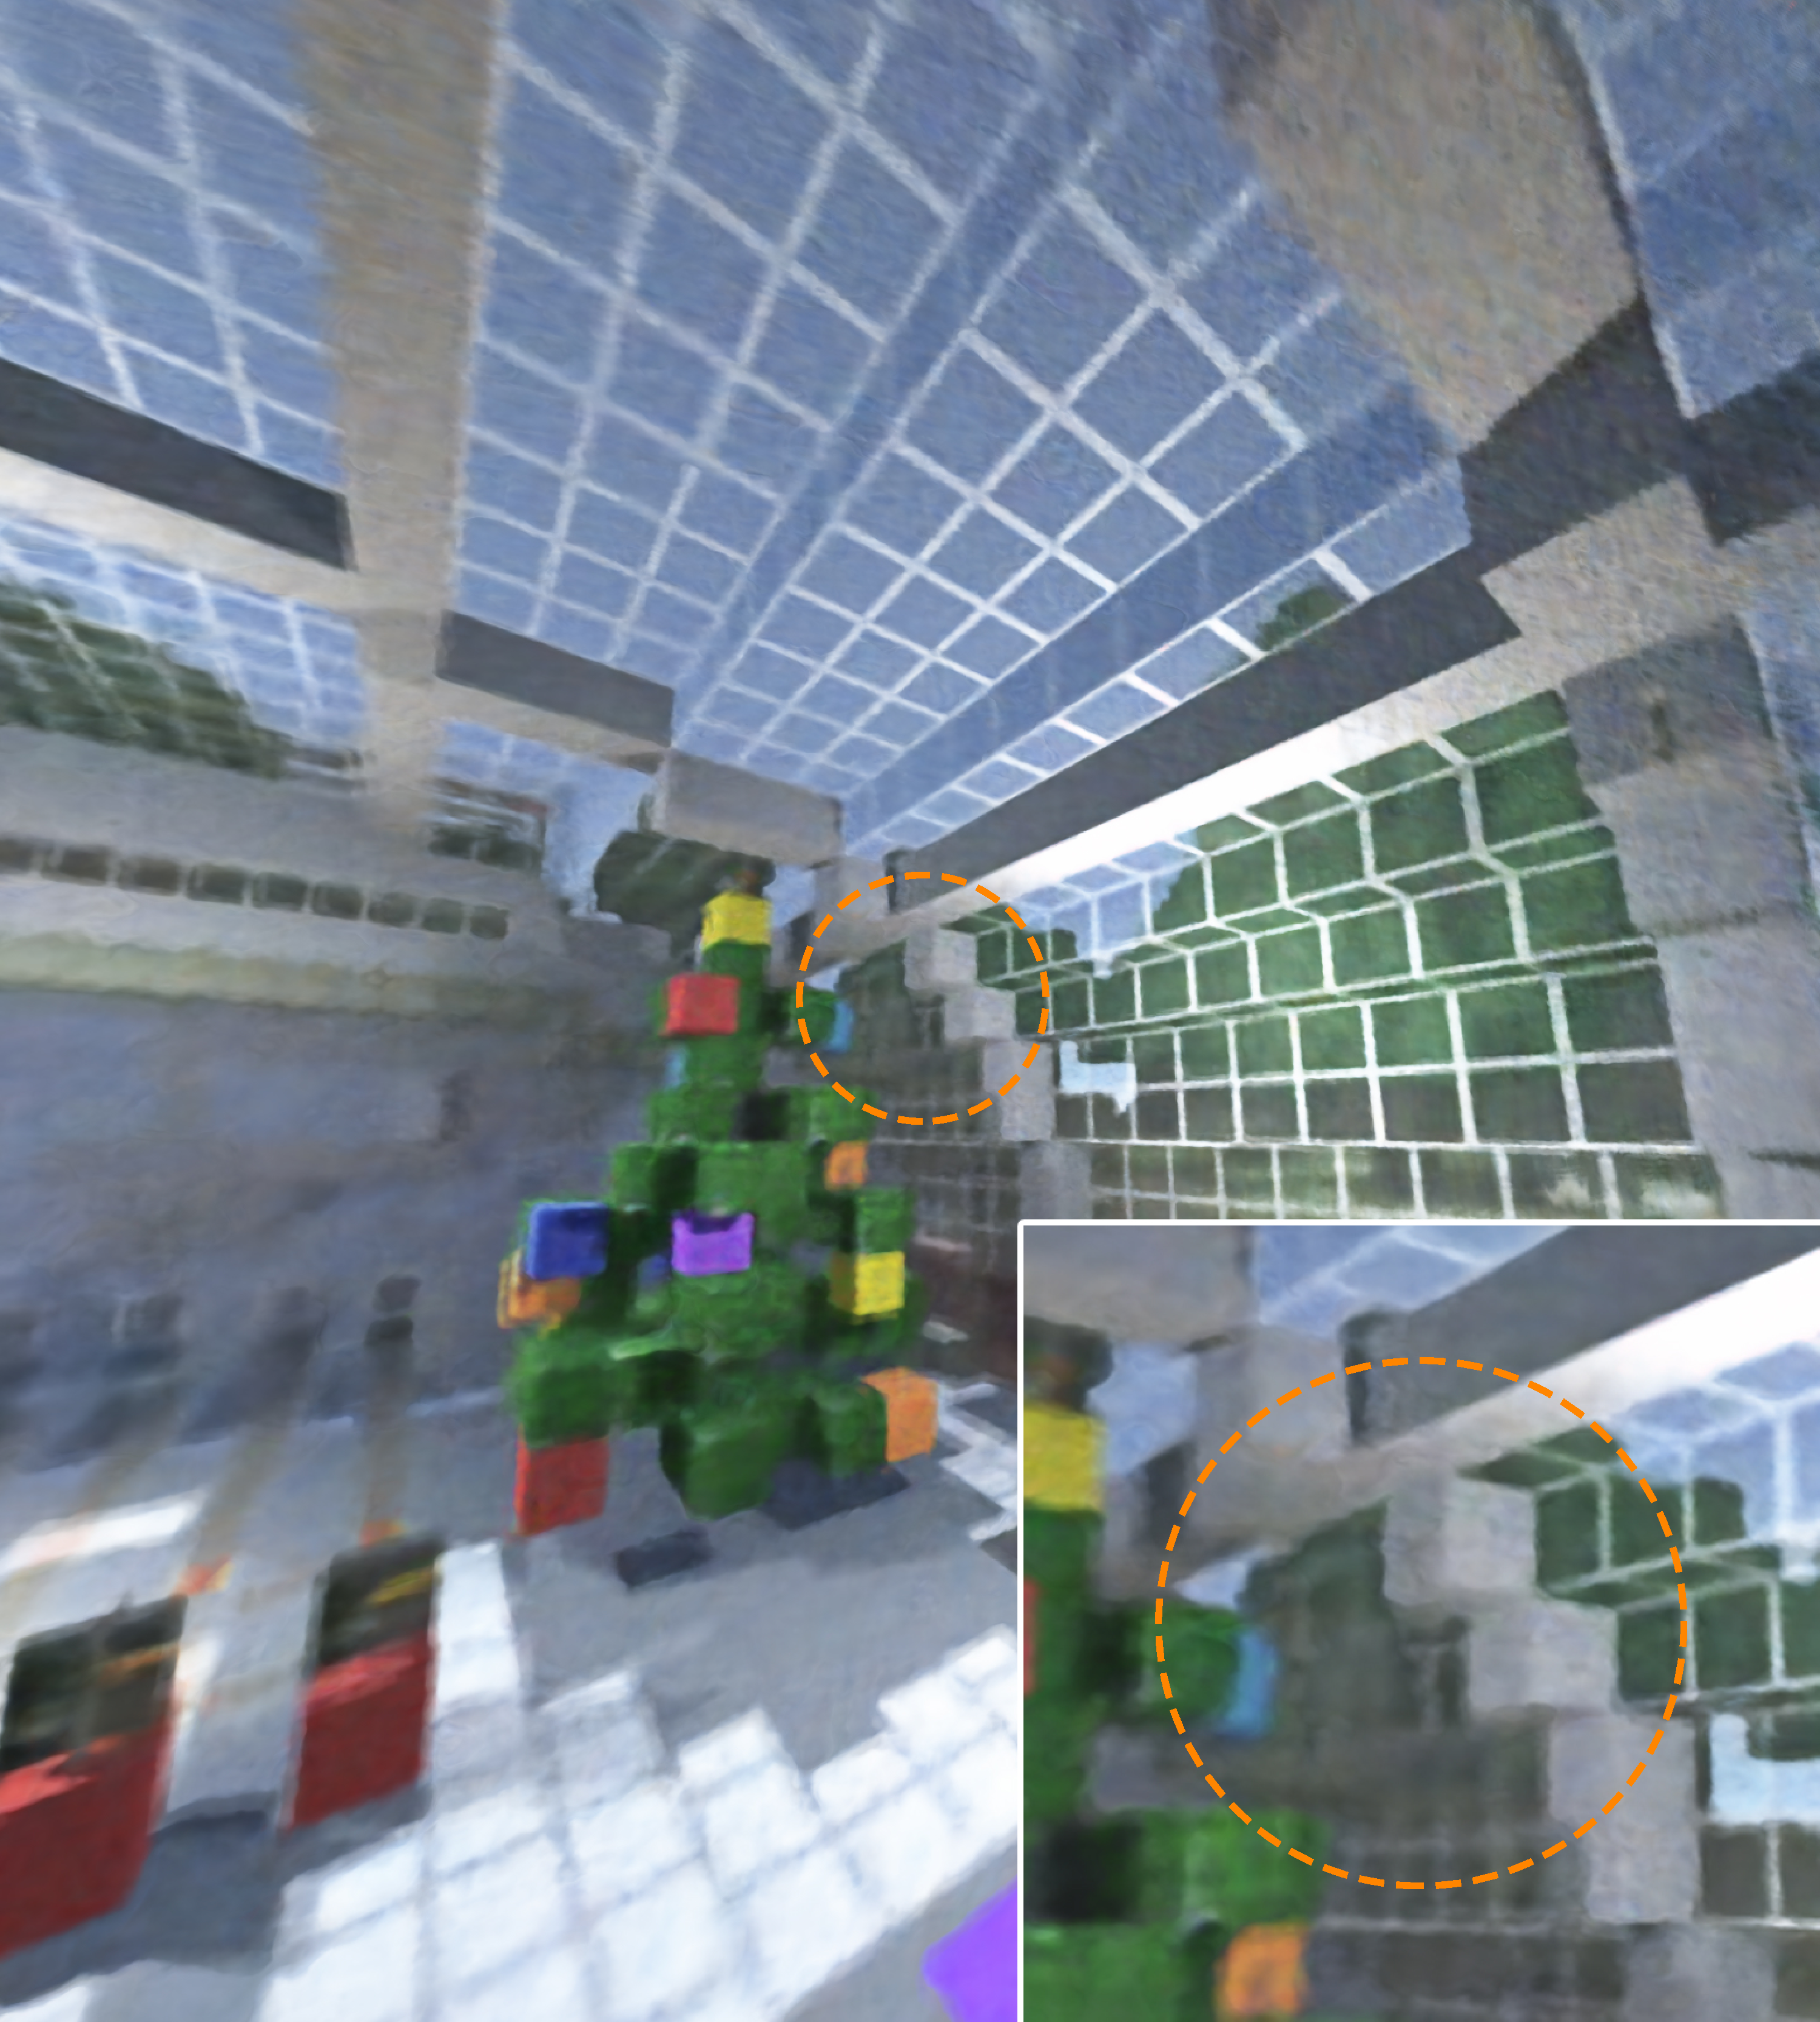
\includegraphics[width=0.96\linewidth]{TOG/figs/mc_nerf3_inset.pdf}}
        
        \subfloat[bedroom scene (\textbf{NeRF})]{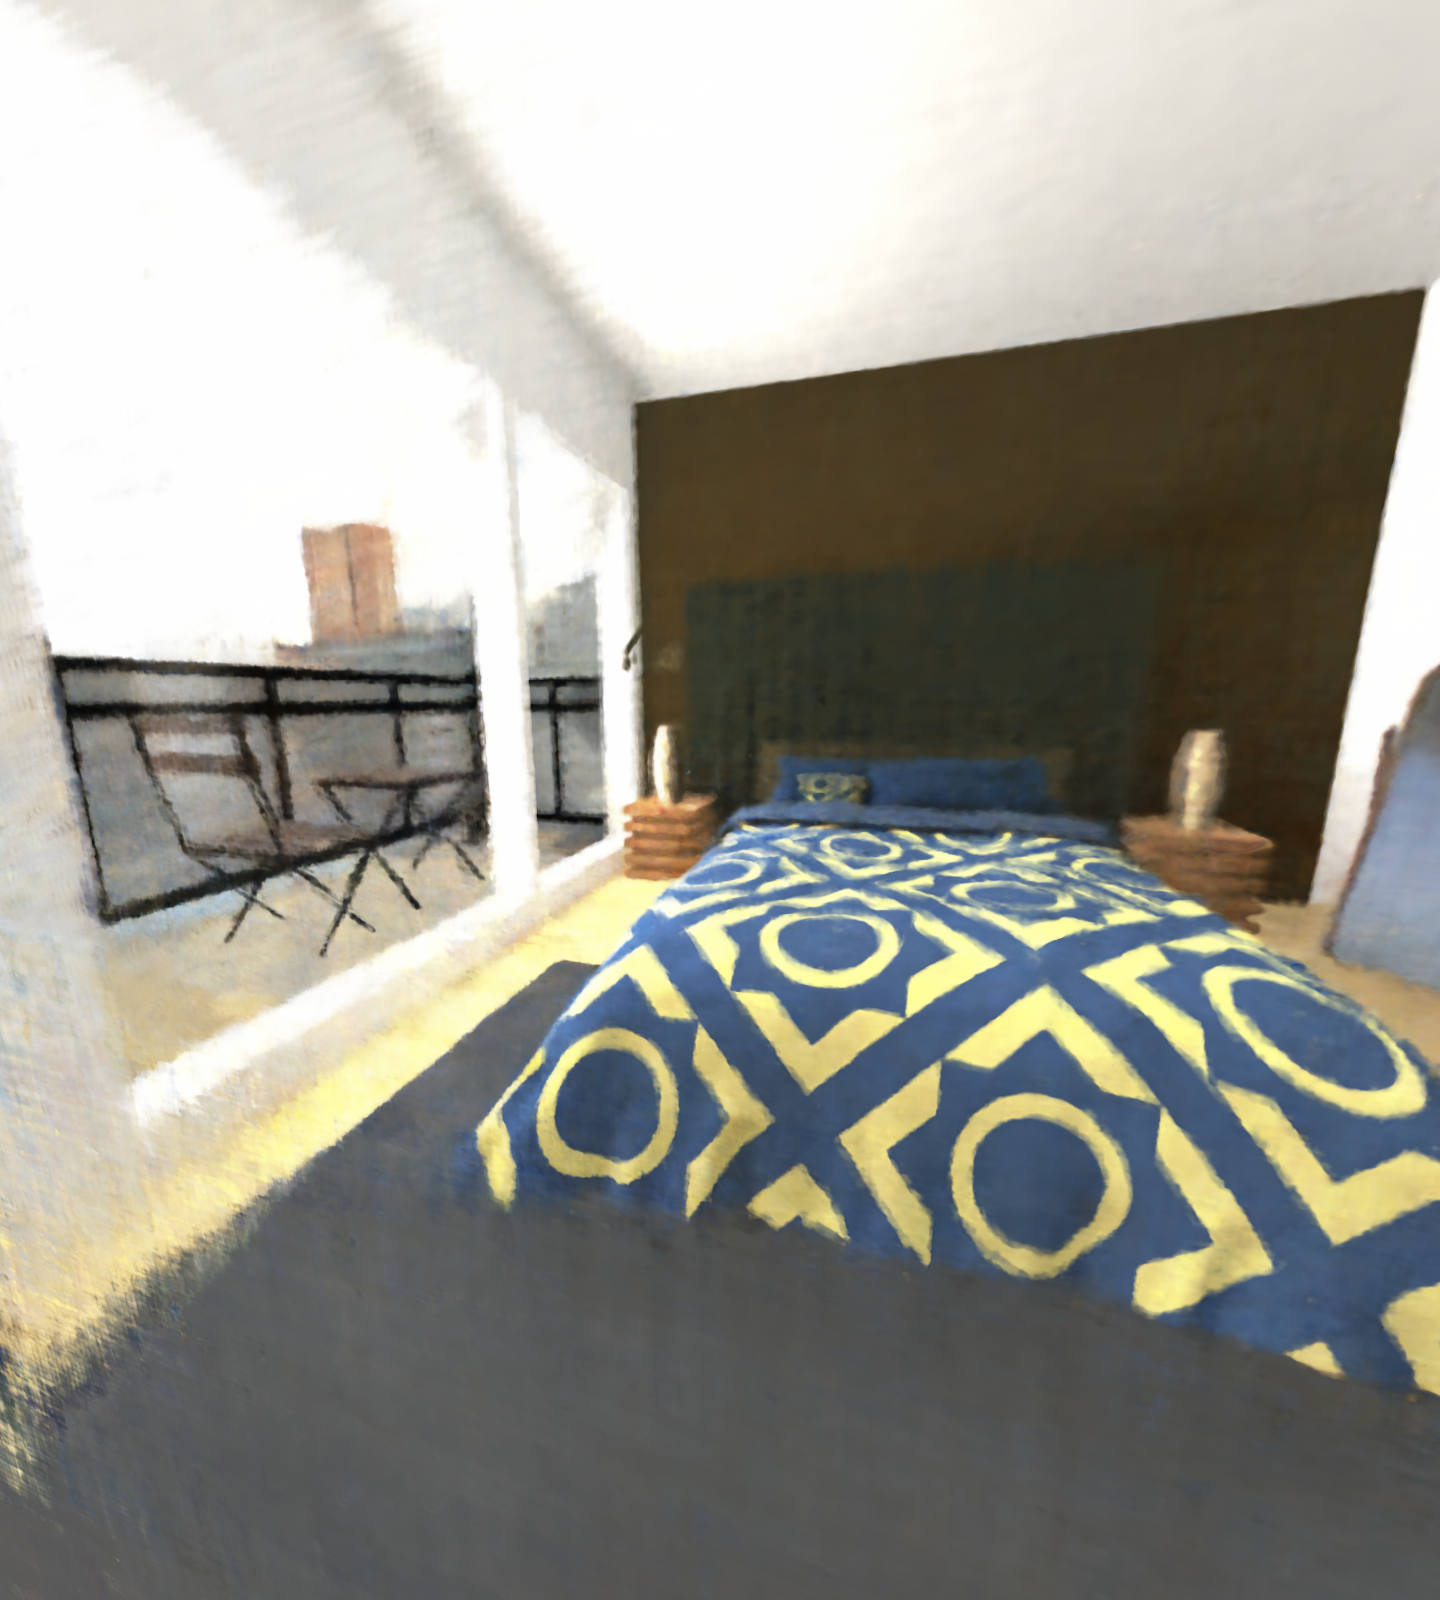
\includegraphics[width=0.96\linewidth]{TOG/figs/bed_nerf0.png}}      
    \end{minipage}    
    
    \caption{Comparing our synthesis method (2nd column) with full resolution (1st column) rendering and NeRF (3rd column).}
    % {\zh{add inset for 2nd and 3rd col}}
    \label{fig:results:comparison}
\end{figure*}

\begin{figure*}[htb]
    \centering
    \begin{minipage}{0.32\linewidth} %full res
        
        \subfloat[gallery scene (\textbf{GT})]{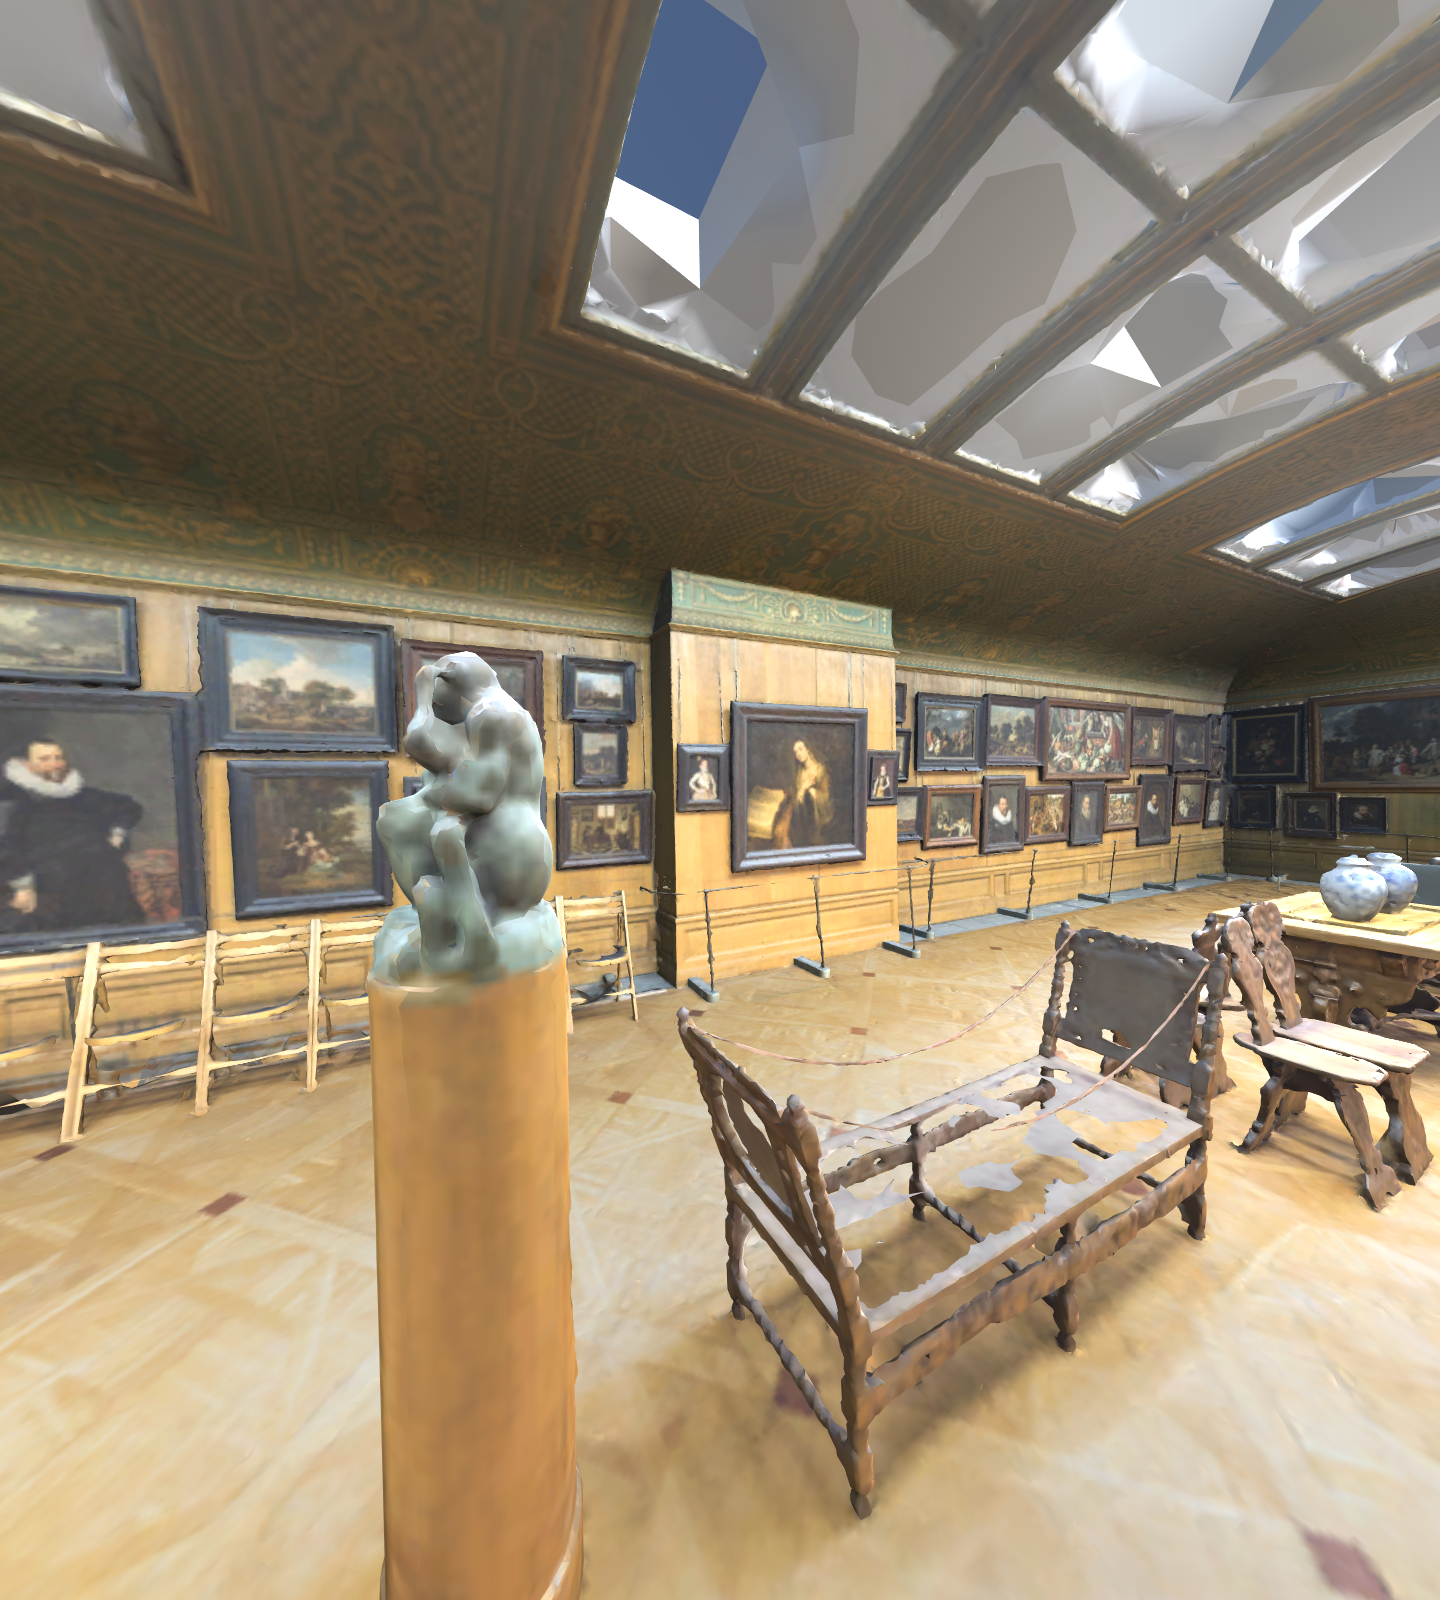
\includegraphics[width=0.96\linewidth]{TOG/figs/gallery_GT_view_0001.png}}
    \end{minipage}
    \begin{minipage}{0.32\linewidth} %ours
        
        \subfloat[gallery scene (\textbf{OUR})]{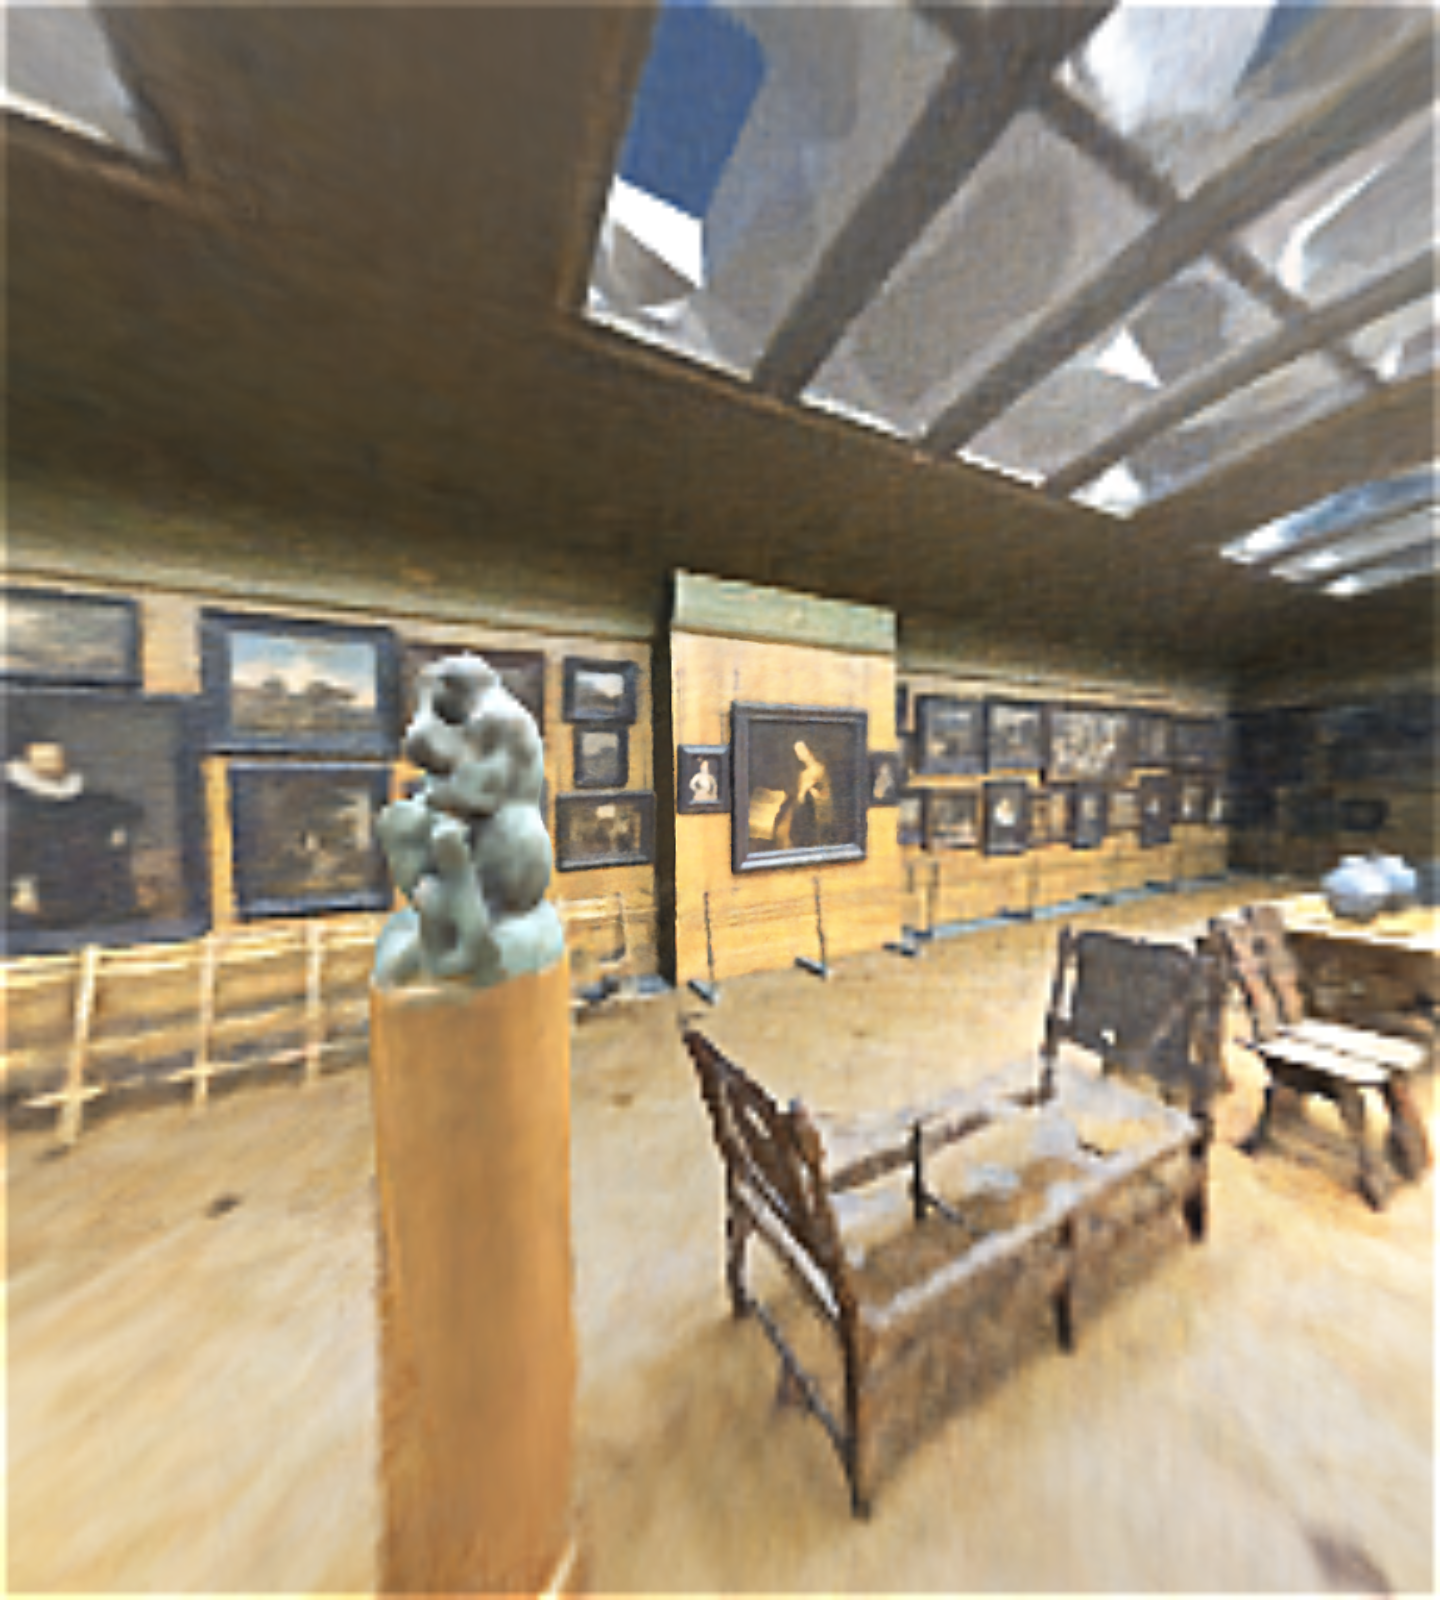
\includegraphics[width=0.96\linewidth]{TOG/figs/gallery_our_001.png}}                
    \end{minipage}
    \begin{minipage}{0.32\linewidth} % NERF
        
        \subfloat[gallery scene (\textbf{NeRF})]{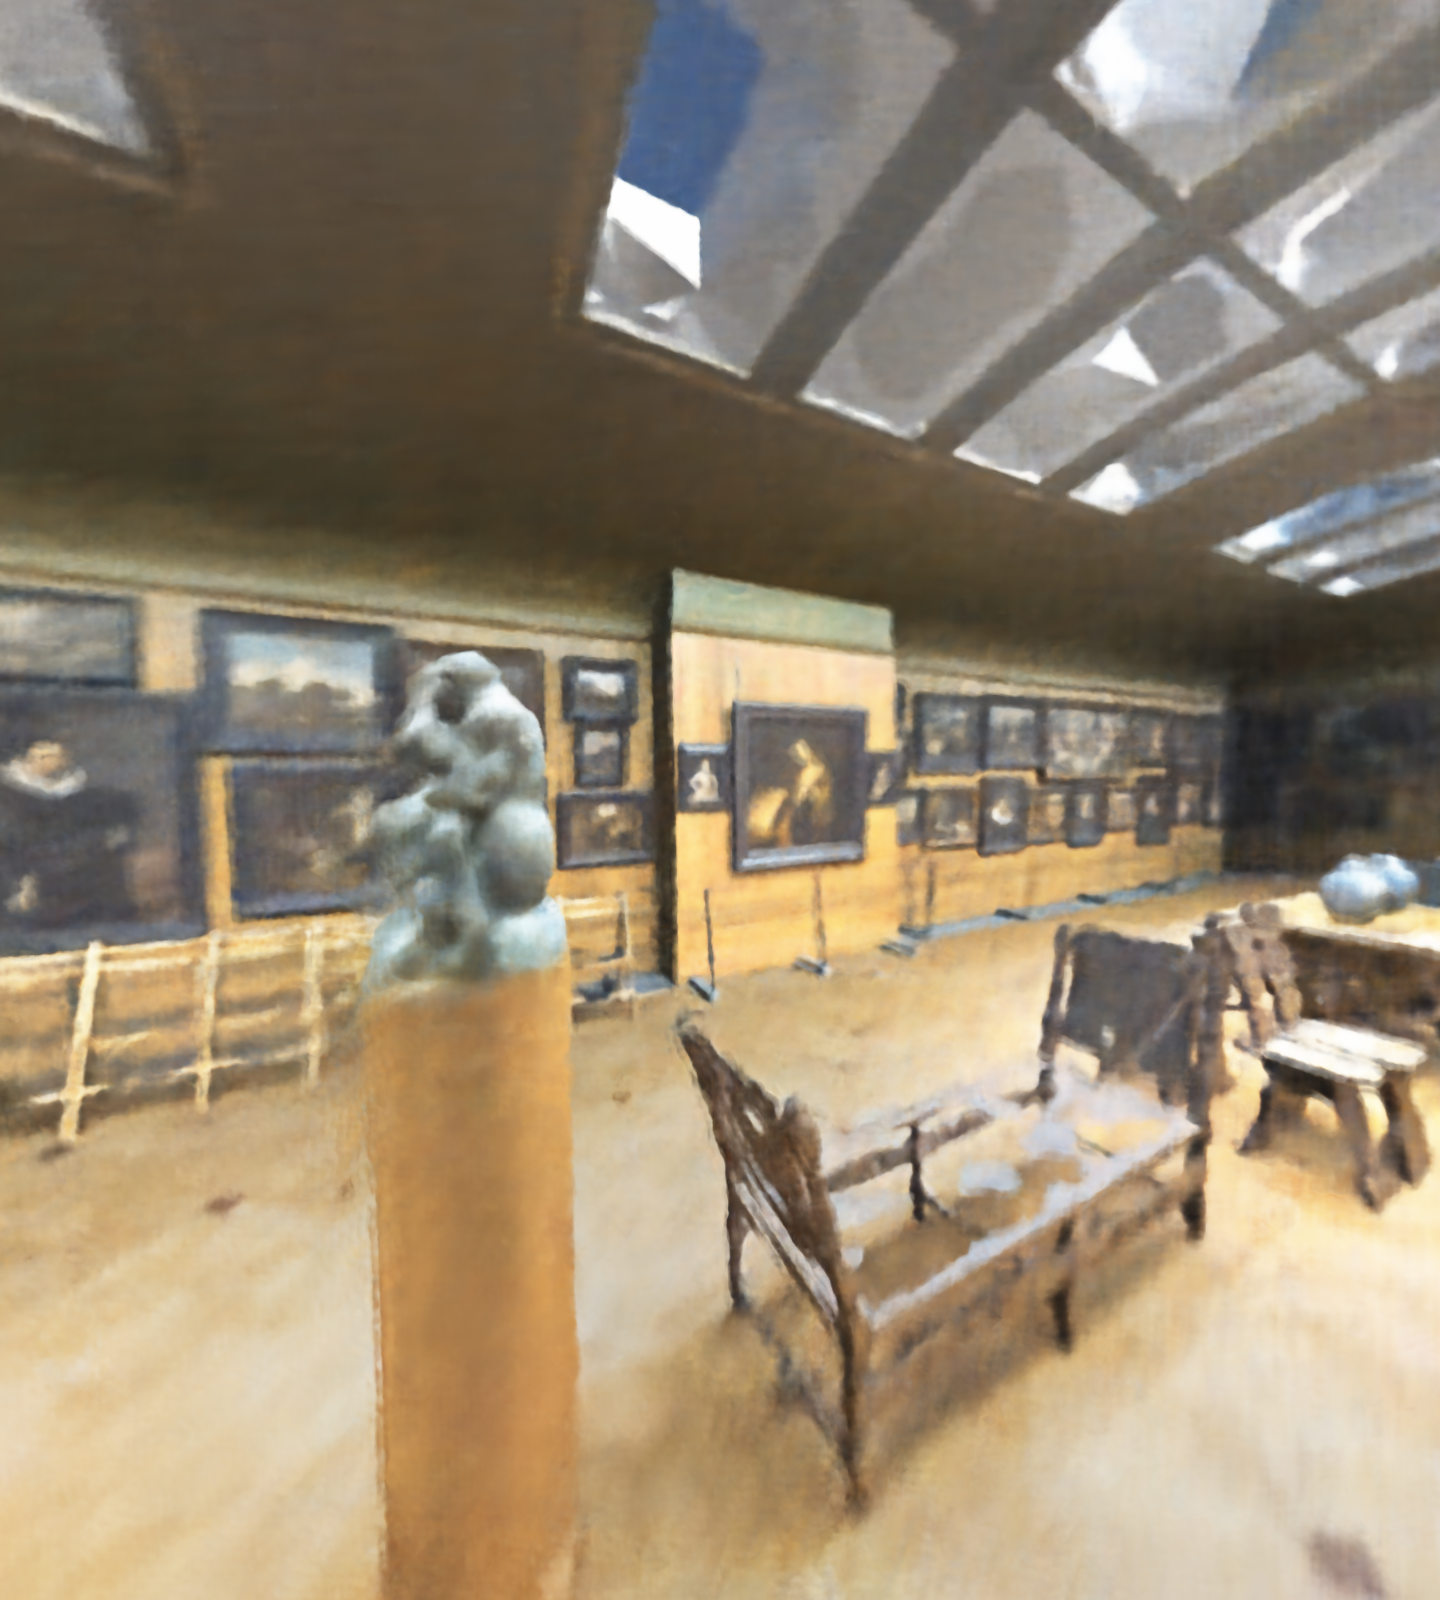
\includegraphics[width=0.96\linewidth]{TOG/figs/gallery_NeRF_001.png}}        
    \end{minipage}    
    
    \caption{Comparing our synthesis method (2nd column) with full resolution (1st column) rendering and NeRF (3rd column). (Cont.).}
    % {\zh{add inset for 2nd and 3rd col}}
    \label{fig:results:comparison2}
\end{figure*}
\paragraph{Environment}
The system was implemented through OpenGL framework using CUDA and accelerated by TensorRT with Intel(R) Xeon(R) Gold 6230R CPU @ 2.10GHz (256GB RAM) and one NVIDIA GTX 3090 graphics card.
For each scene, we trained around 200 epochs for experiment use (about a day).